\section{[Complete] Preventing Current Overload on the Cortex}

\begin{figure}[h]
    \centering
    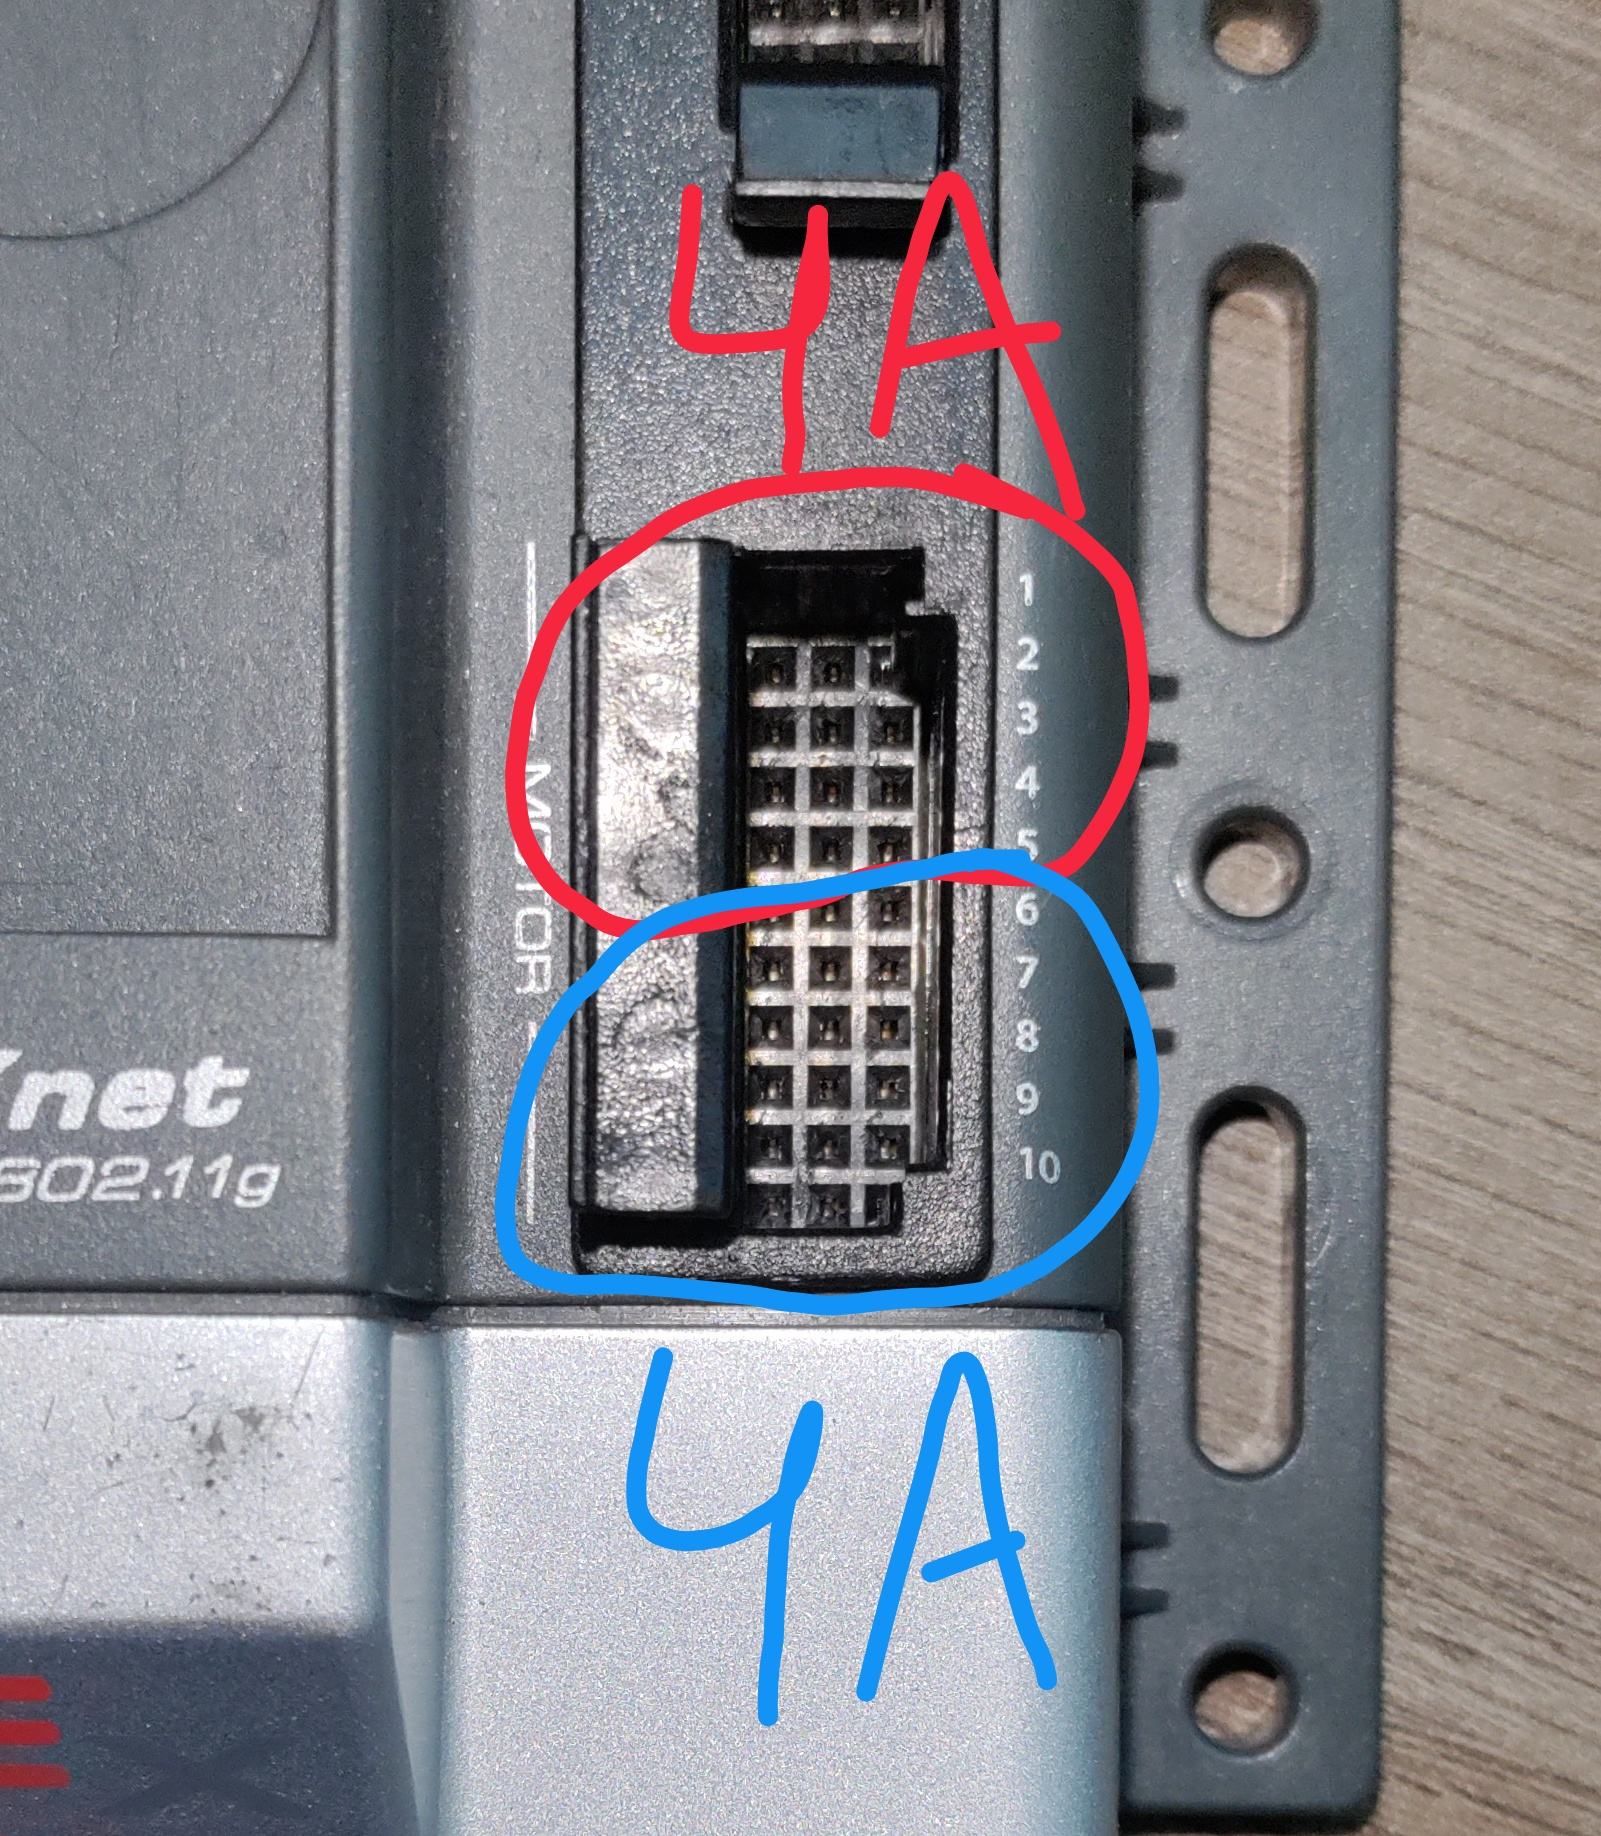
\includegraphics[width=\textwidth,height=9cm,keepaspectratio=true]{MotorWiring/MotorBreakers}
    \caption{
        Each colored circle represents a seperate 4-amp thermal breaker on ports 1-5, 6-10.
    }
\end{figure}

To prevent the battery and circuit board from frying due to internal resistance, the VEX Cortex has two separate thermal 4-Amp breakers (PTC) on motor ports 1-5 and 6-10 \cite{CortexBreakers}. In addition to this, every 393 motor has its own internal thermal breaker (PTC) to further prevent damage to the motors \cite{MotorBreakers}.

To prevent our breakers from triggering from just a few powered motors, we must evenly spread their connections across ports 1-5 and 6-10, so that a roughtly equal amount of motors are on both sides. In addition to this, we must use at least two motors or a high gear ratio on a high-powered mechanism (i.e. arm) so that their internal breakers so not trigger. With this, motors will never overheat during competition, and the cortex will not unexpectedly shut off all of our motors.
